\section{Results}

\subsection{Distributing Plant Capacity: A Classification of the US Coal Fleet}

While the U.S. has seen a decline in coal electricity production over the past ten years, many studies indicate that coal power must be phased out entirely 
by 2030-2035 if we are to meet environmental, social, political, financial, and energy delivery impacts. A graphical representation of coal plants encodes 
multi-dimensional relationships of these factors, and when looking at distributions of these representations, we can extract relationships present in the original 
column-space of the dataset. These local relationships can provide insights for choosing and evaluating phase-out strategy effectiveness and resource allocation. 
More conventional metrics fall short in capturing the intricate relationships and nuances within this high-dimensional space.

To account for the complexity of the coal phaseout problem, we construct a graph model of the US coal fleet, using over 55 variables in the raw column space 
encompassing environmental, political, financial, and other variables. The graph and resulting groups arise from the structure of our high dimensional data set, 
whose complex relationships are distilled into a more interpretable model. Unlike traditional clustering methods, we use the graph model’s structure to build 
digestible descriptions of these groups. This allows us to illustrate which features connect the coal plants in each group, and compare group profiles across all 
available data fields.

\vspace{\baselineskip}

\highlight{How to interpret the model below:
\begin{itemize}
    \item \textit{Nodes} (circles) represent clusters of similar coal plants.
    \item \textit{Edges} (lines) connect similar clusters based on multidimensional relationships in the data.
    \item \textit{Groups} (connected nodes) make up connected components, or isolated sections of the graph.
\end{itemize}
}
%%%%%%%%%%%



%  ╭──────────────────────────────────────────────────────────╮
%  │ Coal Fleet Partition Fig                                 |
%  ╰──────────────────────────────────────────────────────────╯
\begin{figure}[H]
    %  ╭────────────────────────────────────────────────────────────────────────────────────────╮
%  │  custom colors defined based on matplotlib coolwarm colorscheme used in the mapper     |
%  ╰────────────────────────────────────────────────────────────────────────────────────────╯

\usetikzlibrary{positioning}

\definecolor{Group2}{HTML}{7497F5} % Pastel Blue
\definecolor{Group6}{HTML}{94B5FE}
\definecolor{Group5}{HTML}{B4CDFA} % Sky Blue
\definecolor{Group0}{HTML}{D0DAE9} % Pastel Red
\definecolor{Group4}{HTML}{E7D6CC}
\definecolor{Group1}{HTML}{F5C1A8}
\definecolor{Group7}{HTML}{F5A182} % Light Peach
\definecolor{Group3}{HTML}{EA7B60}

\centering
  \includesvg[inkscapelatex=false,width=1\columnwidth]{temp_map.svg}
  
  \centering
    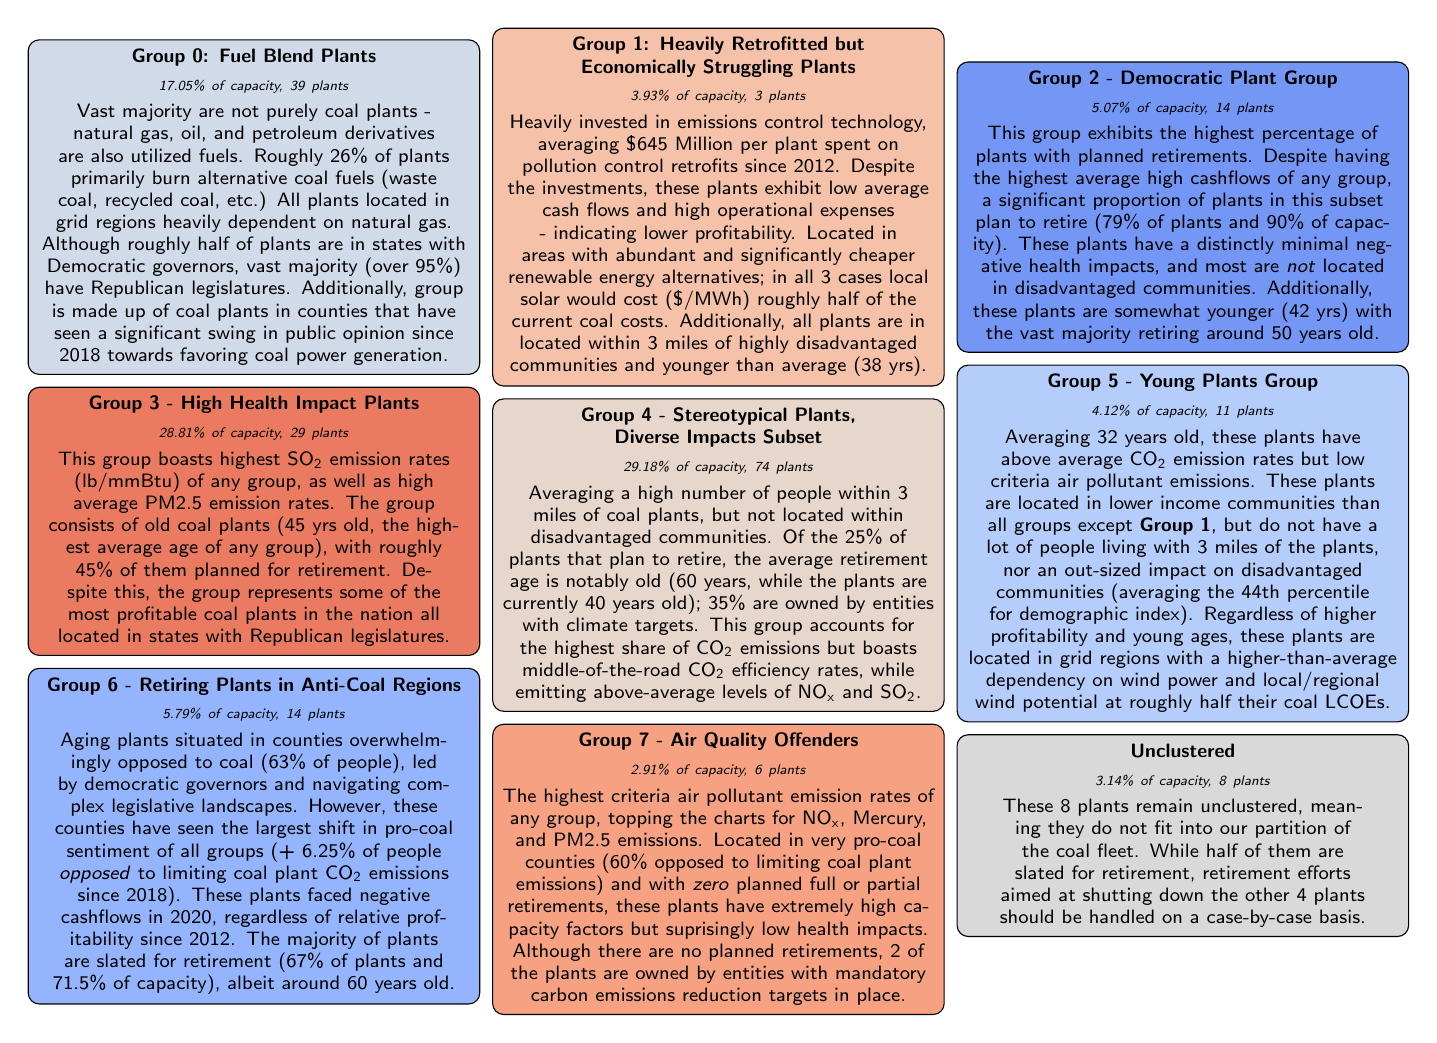
\begin{tikzpicture}[node distance=0.15cm,
    % CHANGE MINIMUM HEIGHT TO MODIFY COLUMN STAGGER
      box/.style={draw, rounded corners, text centered, text width=5.5cm, minimum height=2cm, font=\scriptsize\sffamily},
      title/.style={font=\bfseries\small\sffamily},
      subtitle/.style={font=\footnotesize\sffamily}]


      % Box 1
      \node [box, fill=Group0] (box1) {%
        \textbf{Group 0: Fuel Blend Plants} \\[2pt]
        \textit{\tiny 17.05\% of capacity, 39 plants} \\[2pt]
        Vast majority are not purely coal plants - natural gas, oil, and petroleum derivatives are also utilized fuels. Roughly 26\% of plants primarily burn alternative coal fuels (waste coal, recycled coal, etc.) All plants located in grid regions heavily dependent on natural gas. Although roughly half of plants are in states with Democratic governors, vast majority (over 95\%) have Republican legislatures. Additionally, group is made up of coal plants in counties that have seen a significant swing in public opinion since 2018 towards favoring coal power generation.
      };

      % Box 2
      \node [box, right=of box1, fill=Group1] (box2) {%
        \textbf{Group 1: Heavily Retrofitted but Economically Struggling Plants} \\[2pt]
        \textit{\tiny 3.93\% of capacity, 3 plants} \\[2pt]
        Heavily invested in emissions control technology, averaging \$645 Million per plant spent on pollution control retrofits since 2012. Despite the investments, these plants exhibit low average cash flows and  high operational expenses - indicating lower profitability. Located in areas with abundant and significantly cheaper renewable energy alternatives; in all 3 cases local solar would cost (\$/MWh) roughly half of the current coal costs. Additionally, all plants are in located within 3 miles of highly disadvantaged communities and younger than average (38 yrs).
      };

      % Box 3
      \node [box, right=of box2, fill=Group2] (box3) {%
        \textbf{Group 2 - Democratic Plant Group} \\[2pt]
        \textit{\tiny 5.07\% of capacity, 14 plants} \\[2pt]
        This group exhibits the highest percentage of plants with planned retirements. Despite having the highest average high cashflows of any group, a significant proportion of plants in this subset plan to retire (79\% of plants and 90\% of capacity). These plants have a distinctly minimal negative health impacts, and most are \textit{not} located in disadvantaged communities. Additionally, these plants are somewhat younger (42 yrs) with the vast majority retiring around 50 years old. 
      };

      % Box 4
      \node [box, below=of box1, fill=Group3] (box4) {%
        \textbf{Group 3 - High Health Impact Plants} \\[2pt]
        \textit{\tiny 28.81\% of capacity, 29 plants} \\[2pt]
        This group boasts highest SO\textsubscript{2} emission rates (lb/mmBtu) of any group, as well as high average PM2.5 emission rates. The group consists of old coal plants (45 yrs old, the highest average age of any group), with roughly 45\% of them planned for retirement. Despite this, the group represents some of the most profitable coal plants in the nation all located in states with Republican legislatures.
      };

      % Box 5
      \node [box, right=of box4, below=of box2, fill=Group4] (box5) {%
        \textbf{Group 4 - Stereotypical Plants, Diverse Impacts Subset} \\[2pt]
        \textit{\tiny 29.18\% of capacity, 74 plants} \\[2pt]
        Averaging a high number of people within 3 miles of coal plants, but not located within disadvantaged communities. Of the 25\% of plants that plan to retire, the average retirement age is notably old (60 years, while the plants are currently 40 years old); 35\% are owned by entities with climate targets. This group accounts for the highest share of CO\textsubscript{2} emissions but boasts middle-of-the-road CO\textsubscript{2} efficiency rates, while emitting above-average levels of NO\textsubscript{x} and SO\textsubscript{2}.
      };

      % Box 6
      \node [box, right=of box5, below=of box3, fill=Group5] (box6) {%
        \textbf{Group 5 - Young Plants Group} \\[2pt]
        \textit{\tiny 4.12\% of capacity, 11 plants} \\[2pt]
        Averaging 32 years old, these plants have above average CO\textsubscript{2} emission rates but low criteria air pollutant emissions. These plants are located in lower income communities than all groups except \textbf{Group 1}, but do not have a lot of people living with 3 miles of the plants, nor an out-sized impact on disadvantaged communities (averaging the 44th percentile for demographic index). Regardless of higher profitability and young ages, these plants are located in grid regions with a higher-than-average dependency on wind power and local/regional wind potential at roughly half their coal LCOEs.
      };

      % Box 7
      \node [box, below=of box4, fill=Group6] (box7) {%
        \textbf{Group 6 - Retiring Plants in Anti-Coal Regions} \\[2pt]
        \textit{\tiny 5.79\% of capacity, 14 plants} \\[2pt]
        Aging plants situated in counties overwhelmingly opposed to coal (63\% of people), led by democratic governors and navigating complex legislative landscapes. However, these counties have seen the largest shift in pro-coal sentiment of all groups (\textbf{+} 6.25\% of people \textit{opposed} to limiting coal plant CO\textsubscript{2} emissions since 2018). These plants faced negative cashflows in 2020, regardless of relative profitability since 2012. The majority of plants are slated for retirement (67\% of plants and 71.5\% of capacity), albeit around 60 years old.
      };

      % Box 8
      \node [box, right=of box7, below=of box5, fill=Group7] (box8) {%
        \textbf{Group 7 - Air Quality Offenders} \\[2pt]
        \textit{\tiny 2.91\% of capacity, 6 plants} \\[2pt]
        The highest criteria air pollutant emission rates of any group, topping the charts for NO\textsubscript{x}, Mercury, and PM2.5 emissions. Located in very pro-coal counties (60\% opposed to limiting coal plant emissions) and with \textit{zero} planned full or partial retirements, these plants have extremely high capacity factors but suprisingly low health impacts. Although there are no planned retirements, 2 of the plants are owned by entities with mandatory carbon emissions reduction targets in place.
      };

      % Box 9
      \node [box, right=of box8, below=of box6, fill=gray!30] (box9) {%
        \textbf{Unclustered} \\[2pt]
        \textit{\tiny 3.14\% of capacity, 8 plants} \\[2pt]
        These 8 plants remain unclustered, meaning they do not fit into our partition of the coal fleet. While half of them are slated for retirement, retirement efforts aimed at shutting down the other 4 plants should be handled on a case-by-case basis.
      };
      
      % Title
      % \node [title, above=of box1] (maintitle) {\large Summary Title};

\end{tikzpicture}


    \caption{\textbf{Classifying the US Coal Fleet}}
    \medskip
    \footnotesize
    The resulting model has 8 unique groupings of coal plants. While our groupings are derived from every feature of the data set, looking at homogeneous data fields within each group gives a high-level and digestible overview of why certain plants are grouped together. Here, we label the groups based on some defining characteristics for increased interpretability.
    The node coloring corresponds to the percent of coal plants within each node with plans to retire. Nodes with a higher percentage of retiring coal plants are assigned a darker red. The size of each node is proportional to the total amount of carbon dioxide (CO\textsubscript{2}) emissions in 2022 from the coal plants within the node (scaled). 
    Larger nodes indicate a higher cumulative emission of CO\textsubscript{2} from the associated coal plants.
    \label{fig:coal-fleet-partition}
\end{figure}
%%%%%%%%%%%



\subsection{Understanding Tradeoffs}

\begin{figure}[H]
    \includesvg[inkscapelatex=false,width=\linewidth]{svg_figs/heatmap_small.svg}  
    \caption{\textbf{Plant Groups Comparison}}
    \medskip
    \footnotesize
    The heatmap illustrates the landscape of our coal plant groupings, delineating both the similarities and differences between groups. This helps to provide insights into potential barriers and incentives influencing retirement dynamics within each group.
    A subset of variables was chosen to aid in interpretability and readability, see \textit{Link to SIs} for full heatmap on all variables.
    \label{fig:heatmap}
\end{figure}

\subsubsection{Policy Efficacy and Optimizing Resource Allocation}



%  ╭──────────────────────────────────────────────────────────╮
%  │ Shortest Path Graphs Fig                                 |
%  ╰──────────────────────────────────────────────────────────╯
\begin{figure}[H]
    \centering
    \begin{minipage}{0.5\textwidth}
        \includesvg[inkscapelatex=false,width=\linewidth]{svg_figs/group3_path.svg}  
        \subcaption{\textbf{Group 3} - Distance to Sink Nodes}
    \end{minipage}%
    \begin{minipage}{0.5\textwidth}
        \includesvg[inkscapelatex=false,width=\linewidth]{svg_figs/group4_path.svg}  
        \subcaption{\textbf{Group 4} - Distance to Sink Nodes}
    \end{minipage}

    \begin{minipage}{0.25\textwidth}
        \includesvg[inkscapelatex=false,width=\linewidth]{svg_figs/group3_averageCashflow.svg}  
        \subcaption{Average Cashflows}
    \end{minipage}%
    \begin{minipage}{0.25\textwidth}
        \includesvg[inkscapelatex=false,width=\linewidth]{svg_figs/group3_PM2.5.svg}  
        \subcaption{PM 2.5 Emissions}
    \end{minipage}%
    \begin{minipage}{0.25\textwidth}
        \includesvg[inkscapelatex=false,width=\linewidth]{svg_figs/group4_ownership.svg}  
        \subcaption{Municipal Ownership}
    \end{minipage}%
    \begin{minipage}{0.25\textwidth}
        \includesvg[inkscapelatex=false,width=\linewidth]{svg_figs/group4_proCoal.svg}  
        \subcaption{Oppose Regulating Coal}
    \end{minipage}

    \caption{\textbf{Proximity To Retirement}}
    \medskip
    \footnotesize
    \textbf{(a, b)} Employing Dijkstra's algorithm, we determine the shortest path and corresponding distance from sink nodes to every other node in the graph. Nodes where all plants are planned for full retirement (100\% of plants within) are marked as sinks. These nodes are colored blue and labeled with an \textbf{S}. Distances signify the level of similarity; nodes with shorter paths to sinks share more similar attributes. Conversely, nodes with longer distances have more dissimilar characteristics, indicating a greater divergence between the plants contained within them and the attributes of the retiring plants within sink nodes.  This is our approximation for a \textit{coarse-grained} geodesic distance in high dimensional space. \textit{explain edge weighting here as well?}
    The edges in the graph are weighted to indicate the relationships between nodes. Nodes are sized according to the number of plants in each. 
    \textbf{(c, d, e, f)} Nodes are colored by variables that exhibit variance within the group, emphasizing inter-group distinctions. Higher values are assigned a darker red. The color scheme elucidates the spatial dynamics within connected components of the graph, revealing monotonic trends and differences in specific variables as distances from the source nodes increase.
    \label{fig:shortest-path-graphs}
\end{figure}


%%%%%%%%%%%

% Group 3:
% \begin{table}[H]
%     \centering
%     \small
%     \begin{adjustbox}{width=\textwidth}
%       \begin{tabular}{|l | l | l | l | l | l | l | l | l | l |}
%         \toprule
%         \textbf{Plant Name} & \textbf{State} & \textbf{Retirement Date} & \textbf{Ownership Type} & \textbf{Age at Retirement} & \textbf{Capacity Factor} & \textbf{Coal Nameplate (MW)} \\
%         \midrule\midrule
%         Limestone & TX & 2029 & Investor-Owned & 44 & 35\% & 1850 & \\
%         Belle River & MI & 2028 & Investor-Owned & 44 & 56\% & 1395 & \\
%         Welsh & TZ & 2028 & Investor-Owned & 51 & 44\% & 1116 & \\
%         \bottomrule
%     \end{tabular}
%   \end{adjustbox}
%   \caption{Dataset \& Data Sources Breakdown}
% \end{table}